\documentclass[conference]{IEEEtran}
\IEEEoverridecommandlockouts
% The preceding line is only needed to identify funding in the first footnote. If that is unneeded, please comment it out.
\usepackage{cite}
\usepackage{amsmath,amssymb,amsfonts}
\usepackage{algorithmic}
\usepackage[]{algorithm2e}
\usepackage{graphicx}
\usepackage{textcomp}
\usepackage{xcolor}
\def\BibTeX{{\rm B\kern-.05em{\sc i\kern-.025em b}\kern-.08em
    T\kern-.1667em\lower.7ex\hbox{E}\kern-.125emX}}
\begin{document}

\title{Maze Solver
% {\footnotesize \textsuperscript{*}Note: Sub-titles are not captured in Xplore and
% should not be used}
% \thanks{Identify applicable funding agency here. If none, delete this.}
}

\author{\IEEEauthorblockN{Felipe Leivas Machado}
\IEEEauthorblockA{\textit{262528} \\
\and
\IEEEauthorblockN{Priscila Cavalli Rachevsky}
\IEEEauthorblockA{261573} \\
}}

\maketitle

\section{Introdução}
Será apresentado o problema em questão que é dado uma imagem de um labirinto, descobrir o caminho de solução, também será exposto detalhadamente cada passo da implementação do solucionador de labirintos e seus resultados.

\section{Definição do problema}

\subsection{Descrição do problema}
Dado uma imagem que contém um labirinto, deve-se processá-la de modo que encontre a solução do mesmo e gere como saída a imagem com a solução desenhada.
\subsection {Definição do labirinto}
O labirinto deve conter dois círculos, indicando o ponto de início e chegada do labirinto. O solucionador não suporta labirintos rotacionados, desse forma, para melhores resultados se aconselha que o labirinto seja retangular e com paredes paralelas as bordas da imagem.


\section{Solução do problema}
Para resolver o labirinto, foi usado o seguinte pseudocódigo
\begin{verbatim}
Suavização do ruido
Binarização da imagem
Identificação dos pontos de início e
chegada
Remoção dos pontos de início e chegada da
imagem
Identificação das paredes
Unificação de paredes próximas
Redução do labirinto para uma matriz
Resolução do labirinto
Desenhar a solução no labirinto
\end{verbatim}
\subsection{Suavização do ruído}
 Para suavizar o ruido foi usado um filtro gaussiano com um kernel pequeno, por dois motivos, o primeiro para que as paredes não fossem muito suavizadas com o fundo da imagem, o que dificultaria o processo de binarização; em segundo para que os círculos e paredes não se fundissem, o que dificultaria remover os círculos sem remover as paredes próximas a eles.
 \subsection{Binarização}
 Como a imagem de entrada é praticamente uma imagem linear, fundo branco e as paredes do labirinto com cores escuras, a binarização foi simples. Bastou tornar a imagem original em uma de tons de cinza e usou-se o threshold para a binarização com um valor fixo, encontrado após várias tentativas.

\subsection{Identificação dos pontos de início e chagada}
Para isso foi usado o Hough para detectar os círculos. Para acelerar a busca, limitou-se o tamanho máximo e mínimo do raio do círculo, pois os círculos não são muito grandes já que eles precisam ser menor que o largura do caminho do labirinto. Detectando os dois círculos se assume que o maior é o ponto de chegada e o menor o ponto de início.

\subsection{Remoção dos pontos de início e chagada na imagem}
Para que os círculos não atrapalhassem a busca pelas paredes do labirinto, eles foram removidos. Para isso, removeu-se um círculo com o raio maior do que o círculo encontrado, porque os círculos nas imagens podem ser defeituosos, já que podem ser feitos a mão. O raio do circulo removido é uma porcentagem da imagem.
\subsection{Identificação das paredes}
Para identificar as paredes do labirinto, também foi usado Hough. Como as paredes são perpendiculares e paralelas entre si, foi usado um espaço de busca divido em 90º graus. Com a equação gerada por Hough e com base na imagem, se detectou os pontos iniciais e finais de cada linha gerada por Hough, essas linhas representam as paredes.
\subsection{Unificação de paredes próximas}
O algoritmo de Hough nem sempre retorna uma linha representando uma parede, as vezes o retorno é um conjunto de linhas para representar-la, principalmente quando as paredes são largas e extensas, como as paredes externas, sendo assim, era preciso unifica-las.

Então para unifica-las, primeiramente se separou as linhas em dois grupos, as das paredes horizontais e as das verticais. Depois se pegava uma linha e analisava, no caso de uma linha horizontal, dentre as outras linhas horizontais as que tinham o \(y\) parecido com a linha original e que tinha o valor de \(x\) uma de suas extremidades dentro, ou muito perto, dos valores de \(x\) da linha original. Então se atualizava o valor das extremidades com a nova linha e seguia até passar por todas as linhas.

Se uma linha tivesse no mesmo \(y\) da original mas não no intervalo de \(x\) se adicionava num conjunto de que ainda seria possível "alcançar" ela caso outras linhas fossem adicionadas a essa linha estendendo seu comprimento. E sempre que as extremidades mudavam, esse conjunto de linhas possíveis era adicionado no conjunto de linhas. O mesmo se aplica para as linhas verticais, só mudando os eixos.

\subsection{Redução do labirinto para uma matriz}
Agora contendo as linhas representando as paredes, tentou-se deixar as linhas, que fossem na mesma orientação e tivessem o \(x\) ou \(y\) parecidos, com o mesmo valor, dessa forma essas paredes ficariam na mesma linha ou coluna da matriz quando acontecesse a redução, e não haver falsos buracos.

Depois que as linhas próximas foram padronizadas, se viu a menor distância entre linhas horizontais ou verticais, e isso se definiu o tamanho do bloco. Então a imagem foi discretizadas em blocos de \(tamanho\_do\_bloco X tamanho\_do\_bloco\). Se um bloco tivesse uma parede, aquele bloco inteiro virava uma parede, se naquele bloco tivesse o centro de um dos pontos de inicio ou chegada, aquele bloco virava o bloco de começo ou fim. Senão era um bloco livre, onde o caminho da solução poderia passar.
\subsection{Resolução do labirinto}
Com uma matriz representando o labirinto, foi usado o algoritmo A* para resolver o caminho do ponto de inicio ao ponto de chegada do labirinto.
\subsection{Desenhar a solução no labirinto}
Tendo o caminho gerado pelo passo anterior e sabendo que a solução só pode andar para 4 direções, bastou desenhar uma reta do ponto médio de cada ponto até o ponto médio do próximo ponto na solução.

\section*{Resultados experimentais}
Segue em anexo as imagens de saída do solucionador de labirintos, nas quais em rosa está o caminho encontrado como solução.
\begin{figure}[h!]
   \centering
    {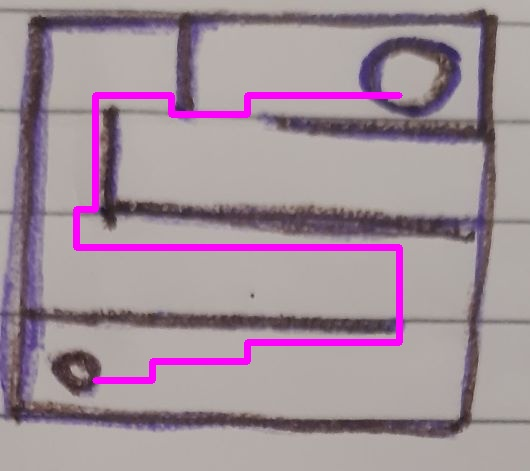
\includegraphics[scale=0.25]{solutioneasy.jpg}}
\end{figure}
\begin{figure}[h!]
   \centering
    {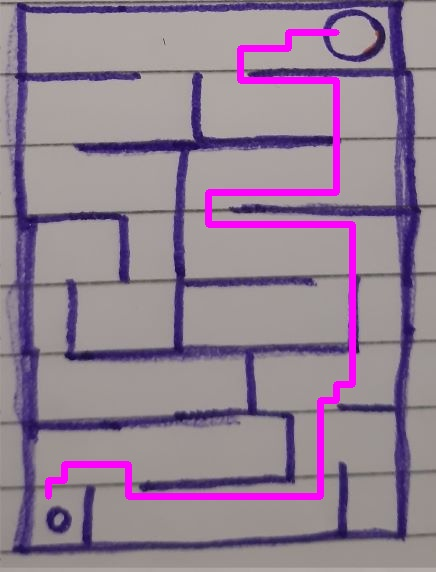
\includegraphics[scale=0.3]{solutionmedium.jpg}}
\end{figure}
\begin{figure}[h!]
   \centering
    {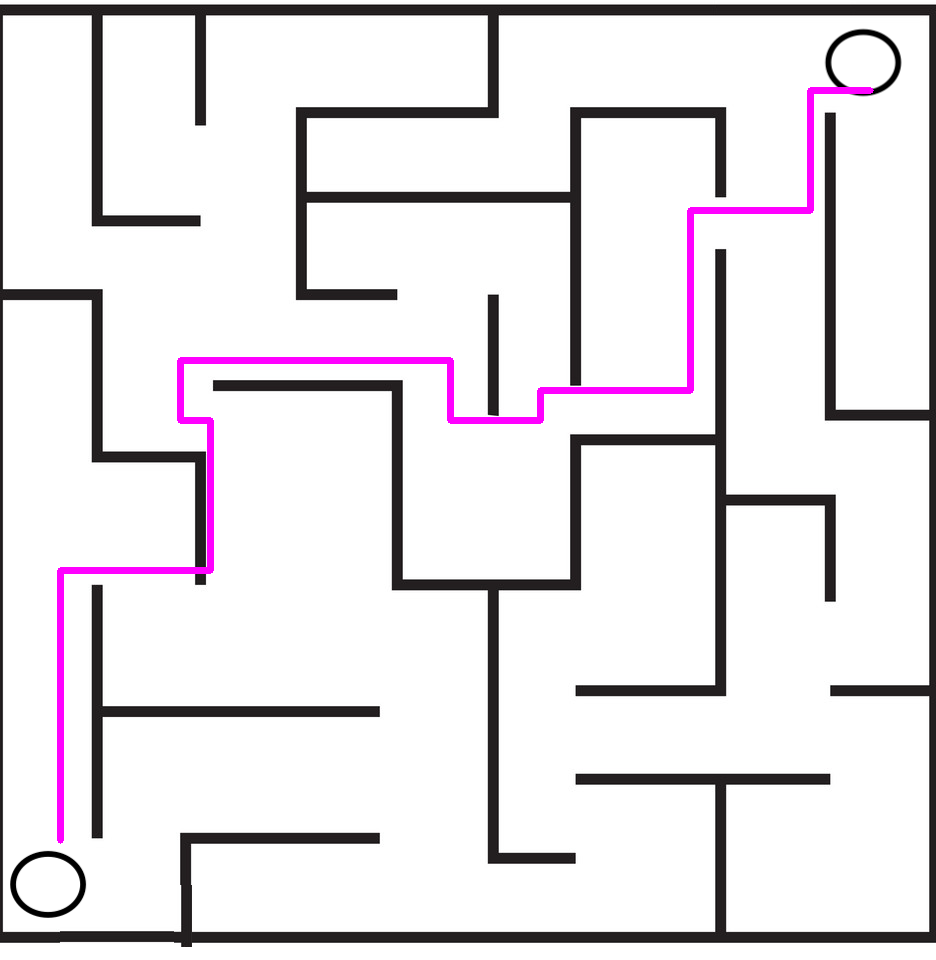
\includegraphics[scale=0.15]{solutionhard.png}}
\end{figure}
\begin{figure}[h!]
   \centering
    {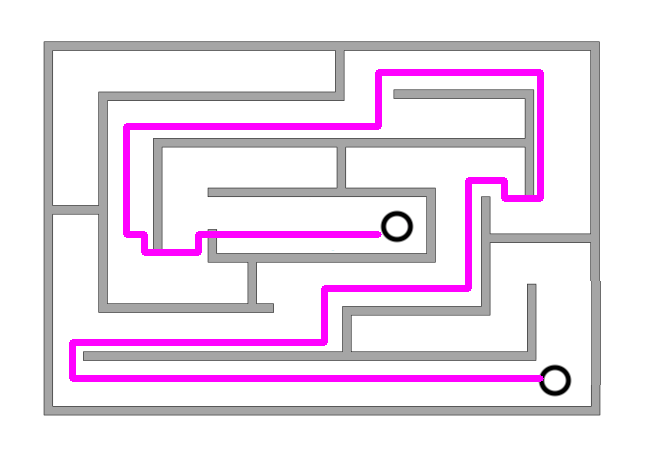
\includegraphics[scale=0.3]{solutionlab2.png}}
\end{figure}
\begin{figure}[h!]
   \centering
    {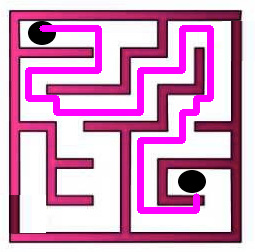
\includegraphics[scale=0.5]{solutionlab3.png}}
\end{figure}

\section*{Conclusão}
A parte de processar a imagem e conseguir coletar os círculos e linhas foi relativamente tranquilo, porque os autores já tinham a base teórica bem consolidada e também já haviam implementado outra ferramenta na mesma cadeira que usava Hough, dessa forma, puderam aproveitar conceitos e até mesmo código.

Transformar a imagem em uma matriz foi onde os autores encontraram maior dificuldade na implementação, mesmo coletando com facilidade os elementos do labirinto, foi complexo descobrir o tamanho dos blocos. Porque se era de tamanho muito grande, poderia desconsiderar alguns espaços entre paredes por serem menores que bloco. Já quando o bloco era de tamanho pequeno, nos casos que a parede não chegava a encostar na outra, mas claramente não era um espaço possível para o caminho, na matriz considerava aquele bloco não sendo parede.


\begin{thebibliography}{00}
\bibitem{b1} https://docs.opencv.org/3.4/d9/db0/tutorial_hough_lines.html

\bibitem{b2} https://docs.opencv.org/3.4/d4/d70/tutorial_hough_circle.html

\bibitem{b3} https://www.laurentluce.com/posts/solving-mazes-using-python-simple-recursivity-and-a-search/
\end{thebibliography}

\end{document}
